\chapter{Exigências Gerais}
\section{Conteúdo}

	O conteúdo do site é de autoria pessoal. Todas as fotos são do portfólio da fotógrafa a mesma disponibiliza e cede os direitos de utilização de imagens para este projeto, com citação a devida citação.
	fotografias: Ester Campos.

\section{HTML5 e CSS}

	Neste projeto foram utilizados $HTML5$ e $CSS$ um dos exemplos para utilização da $CSS$ podem ser conferidos no item $Layout$.
	
     
\section{Framework}

	Foi utilizado o framework Bootstrap seguindo uma das recomendações.

\section{Layout}
	Conforme indicado pelo docente uma das páginas do projeto precisa ser totalmente responsiva. Desta forma apresentamos a página $index.html$.
	
	Não utilizamos $templates$ prontos. Nesta página fazemos utilização de $CSS$.
	
\begin{lstlisting}
<link href="assets/libs/bootstrap/css/bootstrap.css" rel="stylesheet">
<link href="assets/resources/css/principal.css" rel="stylesheet">
<link href="assets/resources/css/home.css" rel="stylesheet">
\end{lstlisting}	
	
	Esta tela é o primeiro contato que um cliente que esteja visitando a página terá. Por este motivo pensamos em mostrar algumas imagens para que o visitante tenha a sensação de que está no lugar certo. 
	
	Desta forma deixamos na página inicial apenas um $slider$ onde são apresentadas cinco (5) fotos. Este $slider$ foi montado para apresentar uma transição de fotos de maneira simples. O intervalo entre uma foto e outra é feito de modo que apareça um efeito de opacidade.
	
	O efeito de opacidade e transição foi conseguido utilizando $CSS$ $transitions$ seguindo algumas ideias de Rich Bradshaw em seu site \cite{RichBradshaw}.

\subsubsection{HTML e CSS}	
	
	Criamos um arquivo chamado $home.css$ onde estão as configurações $crossfade$ do $css$. São estas configurações as responsáveis pelos efeitos de transição/animação das $5$ imagens. Este efeito se dá por $30s$.
	
	Também foi criado um arquivo chamado $principal.css$ neste, estão as configurações para o menu $menuToggle$ que utilizamos nesta página e que também utilizaremos nas demais páginas deste projeto.
	
	Abaixo um trecho do arquivo $index.html$ onde na $tag$ $<nav>$ adicionamos a classe $menu$ e suas configurações são definidas no arquivo $principal.css$.
	
	
	\begin{lstlisting}
<nav class="menu" id="theMenu">
	<div class="menu-wrap">
		<h1 class="logo"><a href="index.html#home">StudioE</a></h1>
		<i class="fa fa-arrow-right menu-close"></i>
		<a href="index.html"><span>HOME</span></a>
		<a href="galeria.html"><span>AUTORAIS</span></a>
		<a href="cliente.html"><span>CLIENTES</span></a>
		<a href="contato.html"><span>ORCAMENTOS</span></a>
		<a href="contato.html"><span>CONTATO</span></a>
		<a href="about.html">INFORMACOES</a>
		<a href="https://www.facebook.com/estercamposfotografia"><i class="fa fa-facebook"></i></a>
		<a href="#"><i class="fa fa-twitter"></i></a>
		<a href="#"><i class="fa fa-envelope"></i></a>
	</div>
	<!-- Menu button -->
	<div id="menuToggle"><i class="fa fa-bars navicon img-responsive"></i></div>
</nav>
\end{lstlisting}


	Para o ícone do menu, foi configurado no $css$ as seguintes linhas:
	
	\begin{lstlisting}
    #menuToggle {
        position: absolute;
        top: 3px;
        left: 0;
        right: 10;
        z-index: 11;
        opacity: 1;
        text-align: center;
        font-size: 30px;
        color: #000;
        width: 20px;
        height: 20px;
        line-height: 30px;
        padding: -10px;
        cursor: pointer;
        -webkit-transition: all .1s ease-in-out;
        transition: opacity 0.5s;
        -moz-transition: all .1s ease-in-out;
        -ms-transition: all .1s ease-in-out;
        -o-transition: all .1s ease-in-out;
        transition: all .1s ease-in-out;
    }  
\end{lstlisting}


	Ao passar o $mouse$ em cima do ícone mudamos a cor do ícone para cinza claro:
	
	
		\begin{lstlisting}
	   #menuToggle:hover {
        color: #ccc;
        -webkit-transition: all .1s ease-in-out;
        -moz-transition: all .1s ease-in-out;
        -ms-transition: all .1s ease-in-out;
        -o-transition: all .1s ease-in-out;
        transition: all .1s ease-in-out;
    }
\end{lstlisting}
\subsubsection{Teste Webdevelopers}	  

    Utilizamos a extensão para navegador web $Web Developers$ para testar a responsividade desta página. Este teste foi feito utilizando o navegador web $Mozilla$ $Firefox$ $for$ $Linux$ $Mint$ versão $49.0.2$ e $Web$ $Developer$ versão $1.2.11$.
    
    Web Developer é um plugin que "adiciona um menu e uma barra com várias ferramentas de desenvolvimento para web"
    
    
\begin{lstlisting}
    chrome://web-developer/content/generated/view-responsive-layouts.html#content
\end{lstlisting}

	Abaixo listamos duas imagens que mostram um resultado do teste. Mais testes podem ser realizados durante a apresentação deste projeto.

\begin{figure}[!htb]
\setcounter{figure}{0}
\centering
\begin{minipage}{.5\textwidth}
  \centering
  \includegraphics[width=.3\linewidth]{./img/1.png}
  \captionof{figure}{321x480}
\end{minipage}%
\begin{minipage}{.5\textwidth}
  \centering
  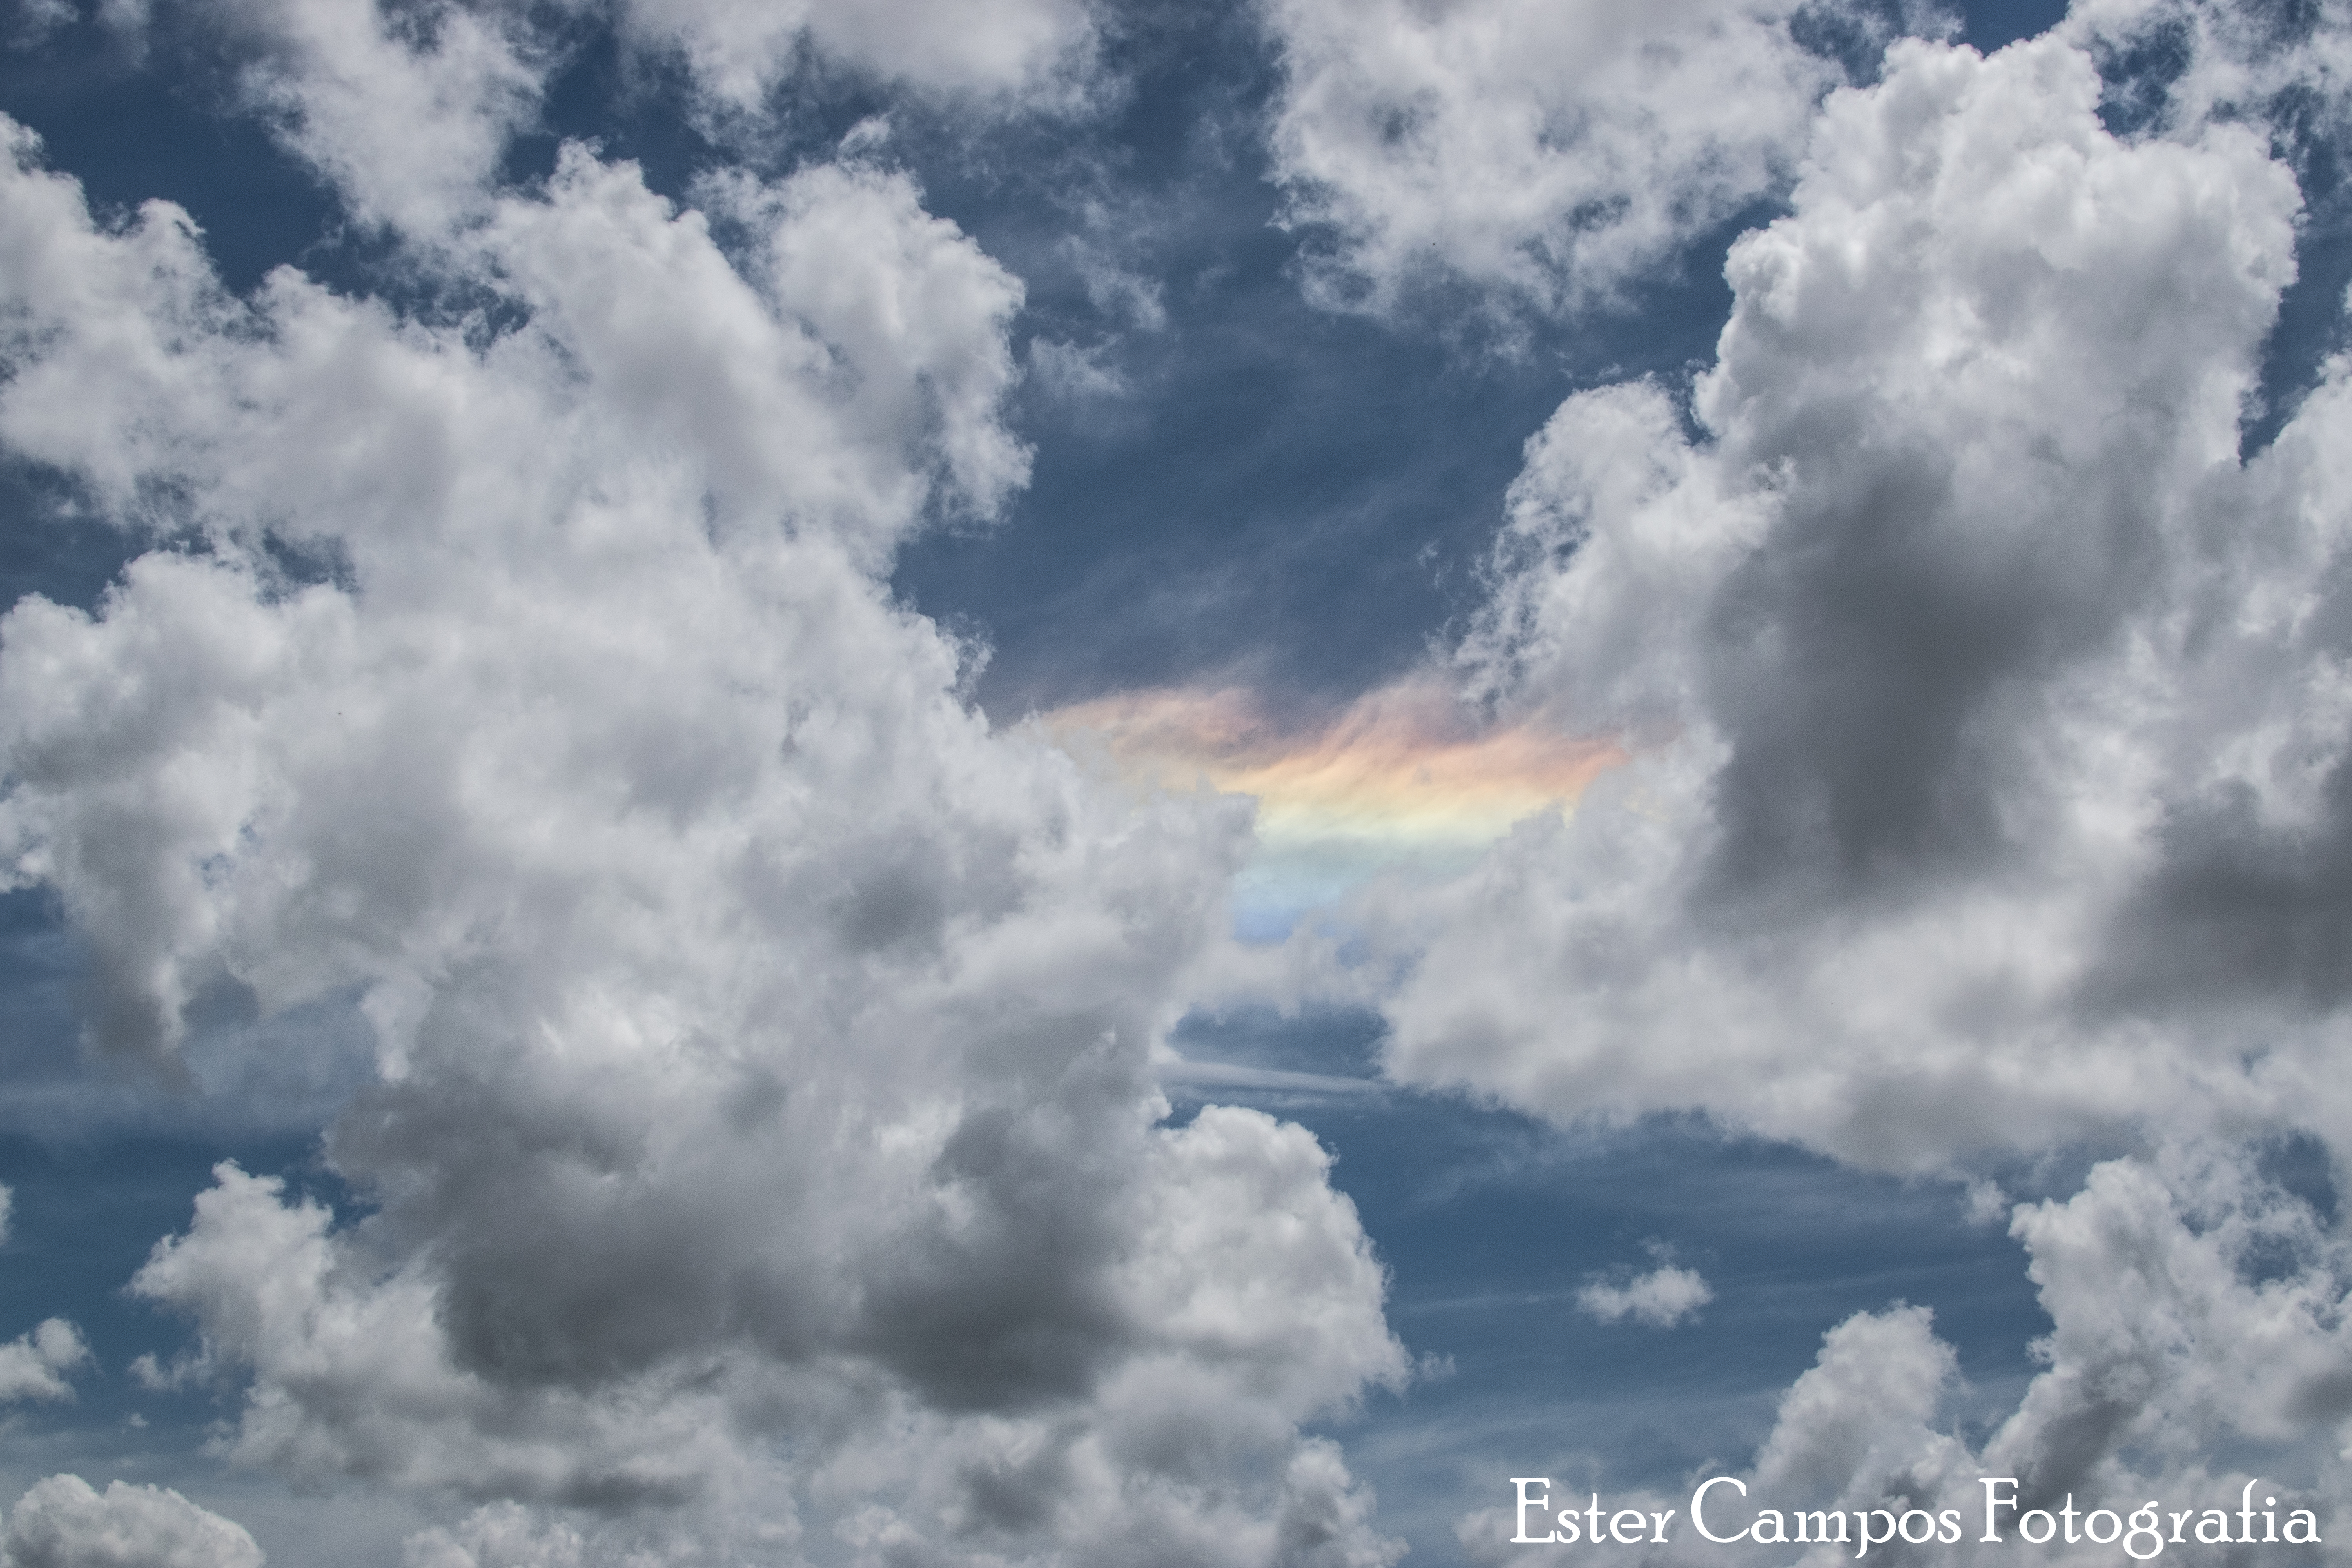
\includegraphics[width=.8\linewidth]{./img/6.png}
  \captionof{figure}{1024x768}
\end{minipage}
\end{figure}